\chapter{Solution Description}
 {\color{red} This section is for decomposing the problem and describing the Methods for each subtask. }

 \section{Coordinate Systems Used}\label{41}
At this stage, two coordinate systems are used: the first is related to the football field, where the top-left corner is considered the point (0, 0), and the second is related to the camera coordinates, in a reference system linked to the far left corner of the field. For given coordinates $X,\;Y$, the transition from one plane to another is carried out according to the following law:

$$
\begin{bmatrix}
\tau_{i}X' \\
\tau_{i}Y' \\
\tau_{i}
\end{bmatrix} = 
\underbrace{ \begin{bmatrix}
a_{1} & a_{2} & b_{1} \\
a_{3} & a_{4} & b_{2} \\
c_{1} & c_{2} & 1
\end{bmatrix} }_{ M } \begin{bmatrix}
X \\
Y \\
1
\end{bmatrix},
$$

where $a_i$ are scaling/rotation elements, $\begin{bmatrix}
    b_2 & b_1
\end{bmatrix}^T$ is the shift vector, and $\begin{bmatrix}
    c_1 & c_2
\end{bmatrix}$ is the projection vector.

To find the true values of $X', Y'$, the resulting vector must be divided by the coefficient $\tau_i$, which is the scaling factor.

As a result, an algorithm was developed using the cv2 library, which takes two arguments as input: four initial coordinates (x, y), which indicate the initial corners of the rectangle of the transition area, and the second argument - four coordinates that indicate the desired corner coordinates for the output image. The algorithm produces a transformation matrix $M \in \mathbb{R}^{3 \times 3}$, after which the algorithm is sequentially applied to each frame from the initial dataset. As a result, a new dataset is obtained in which for each id, i.e., the recognized object in the frame, new coordinates ($X', Y'$) are obtained. An example visualizing the algorithm's work:

 \begin{figure}[!h]
     \centering
     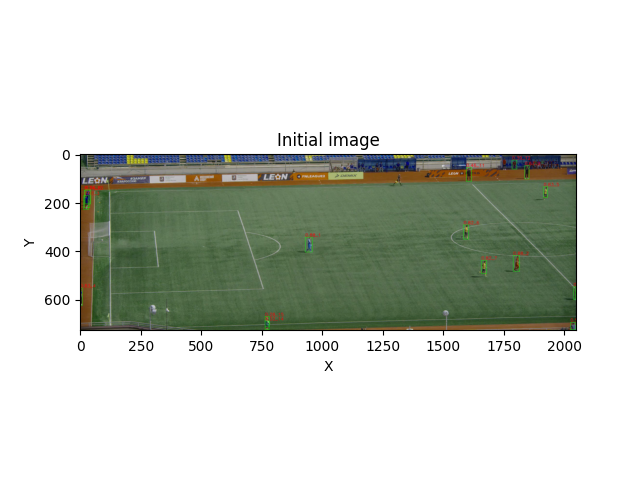
\includegraphics[width=0.8\linewidth]{figures/Initial image.png}
     \caption{Image before transformation of coordinates}
     \label{fig:before-transform}
 \end{figure}

  \begin{figure}[!h]
     \centering
     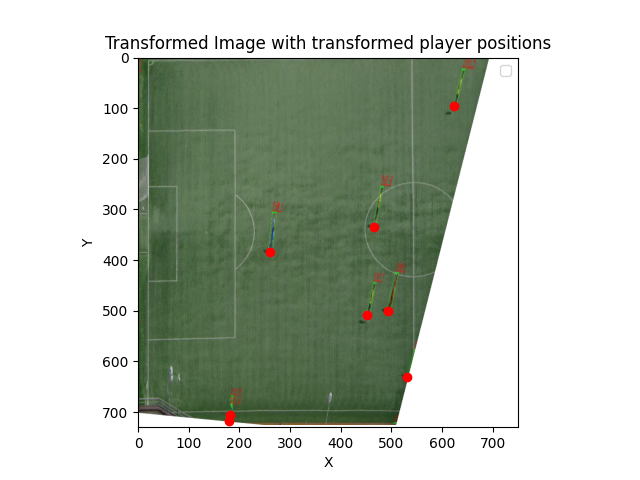
\includegraphics[width=0.8\linewidth]{figures/Transformed Image with transformed player positions.png}
     \caption{Image after transformation of coordinates}
     \label{fig:after-transform}
 \end{figure}


\section{Preprocessing}
\section{Algorithm Development for the Case of Static Players}
There are many solutions for the TSP problem, but there are several key differences between them, the main one being the accuracy of the solution. Some algorithms can solve the problem of finding the minimal closed path exactly, while others do not guarantee the minimal path but are significantly faster. For this specific task, the exact solution option was chosen since the number $n$, i.e., the number of recognized objects in the frame, is small.

Thus, according to the article~\cite{Zhang_2021}, the most optimal option was the dynamic programming method, since among the exact approaches to solving TSP, it showed the highest speed. The implemented algorithm takes one frame with recognized objects, with already transformed coordinates, the transition to which was solved in section \ref{41}, and returns a path that includes the ids of all recognized objects in the frame, in the order that minimizes the Hamiltonian closed path in the graph, whose vertices are the ids, as well as the total path length. For the next task of developing an algorithm for the case of moving players, it will probably be necessary to revise the algorithmic approach to solving the problem. Nevertheless, the dynamic programming approach can be considered successful at this stage.

\section{Environment Simulation}
\subsection{Agent Simulation}
\subsection{Camera Simulation}
\subsubsection{Line - Plane Intersection}
Intersection of a plane with a line:
Let $p_0$ be the camera vector, and $v_0$ be the direction vector of the light ray passing through the camera vector (center of the focal lens).

Then the parametric equation of the line can be defined as:
$$P(t) = p_0 + t \cdot v_0 \qquad \text{($P(t)$ is a point on the line)}$$

We need to find such a $t$ that $P(t)$ lies on a given plane.
Substituting this into the plane equation, we get:
$$a(P0_x + tV0_x) + b(P0_y + tV0_y) + c(P0_z + tV0_z) = d$$

Solving for $t$ ($n$ is the normal vector of the plane):
$$t = \frac{D - nP0}{n \cdot V0}$$

We are interested in $t < 0$ since positive values correspond to the wrong light direction.

\subsubsection{Field of View and Angle of View}
For truthful simulation of field of view and physics of long-focus cameras, work of Matvey Gancev was used. As simulation of physics for camera is a complicated and time-requiring task, with the admition of Matvey Gancev, the simulation code was used. However modeling the camera movement and traversal algorithm are completed without use of intelectual property from other researchers. It is a complicated task to set the angle velocity, thus it can be estimated with a velocity on a euclidean plane. 

Field of View: The calculatePanoramicSystemFOV method calculates the angle of view (FOV) for each camera in the panoramic system and returns a list of camera angles of view for the panoramic system.

The method defines the plane vector and the coordinates and angles of the panoramic system. Then for each camera in the panoramic system, the following occurs:

\begin{enumerate}
    \item The camera coordinates and its angles of view are calculated.
    \item Vectors defining the camera's angles of view are created.
    \item Rotations are applied to the vectors of the camera and the panoramic system.
    \item The intersection point of the line (defined by the camera) with the plane (panoramic system) is calculated.
    \item The camera's angle of view and the main axis of the camera's view are calculated.
\end{enumerate}


1. Calculation of vector a:
$$
\text{vector\_a} = \begin{bmatrix}
1.0 \\
\tan\left(\frac{\text{camera\_width\_angle\_of\_view}}{2}\right) \\
-\tan\left(\frac{\text{camera\_height\_angle\_of\_view}}{2}\right)
\end{bmatrix}
$$

2. Rotation of vector $ \mathbf{a} $:
$$
\mathbf{a} = \left(\mathbf{R}_\text{ps} \cdot \mathbf{R}_\text{c}\right) \cdot \mathbf{a}
$$

Here $ \mathbf{R}_\text{ps} $ and $ \mathbf{R}_\text{c} $ are the rotation matrices for the panoramic system and the camera, respectively.

3. Re-rotation of vectors $ \mathbf{b} $, $ \mathbf{c} $, $ \mathbf{d} $, $ \mathbf{p} $:
\begin{align*}
\mathbf{b} &= \left(\mathbf{R}_\text{ps} \cdot \mathbf{R}_\text{c}\right) \cdot \mathbf{b} \\
\mathbf{c} &= \left(\mathbf{R}_\text{ps} \cdot \mathbf{R}_\text{c}\right) \cdot \mathbf{c} \\
\mathbf{d} &= \left(\mathbf{R}_\text{ps} \cdot \mathbf{R}_\text{c}\right) \cdot \mathbf{d} \\
\mathbf{p} &= \left(\mathbf{R}_\text{ps} \cdot \mathbf{R}_\text{c}\right) \cdot \mathbf{p} 
\end{align*}

Here $ \mathbf{R}_\text{ps} $ and $ \mathbf{R}_\text{c} $ are also the rotation matrices for the panoramic system and the camera.

4. Calculation of point $ \mathbf{t}_0 $:
$$
\mathbf{t}_0 = \mathbf{r}_\text{ps} + \mathbf{R}_\text{ps} \cdot \mathbf{r}_\text{c}
$$

Here $ \mathbf{r}_\text{ps} $ and $ \mathbf{r}_\text{c} $ are the coordinates of the panoramic system and the camera, respectively.

5. Definition of parameters $a_0$, $b_0$, $c_0$, $d_0$, $p_0$:

\begin{align*}
a_0 &= -\frac{\left(\mathbf{v}_\text{plane} \cdot \mathbf{v}_{\text{t}_0}\right) + D} {\left(\mathbf{v}_\text{plane} \cdot \mathbf{v}_a\right)} \\
b_0 &= -\frac{\left(\mathbf{v}_\text{plane} \cdot \mathbf{v}_{\text{t}_0}\right) + D} {\left(\mathbf{v}_\text{plane} \cdot \mathbf{v}_b\right)} \\
c_0 &= -\frac{\left(\mathbf{v}_\text{plane} \cdot \mathbf{v}_{\text{t}_0}\right) + D}{\left(\mathbf{v}_\text{plane} \cdot \mathbf{v}_c\right)} \\
d_0 &= -\frac{\left(\mathbf{v}_\text{plane} \cdot \mathbf{v}_{\text{t}_0}\right) + D}{\left(\mathbf{v}_\text{plane} \cdot \mathbf{v}_d\right)} \\
p_0 &= -\frac{\left(\mathbf{v}_\text{plane} \cdot \mathbf{v}_{\text{t}_0}\right) + D}{\left(\mathbf{v}_\text{plane} \cdot \mathbf{v}_p\right)}
\end{align*}

6. Calculation of the coordinates of the angles of view and the main axis of the camera:
\begin{align*}
\text{fov\_a} &= a_0 \cdot \mathbf{v}_a + \mathbf{v}_{\text{t}_0} \\
\text{fov\_b} &= b_0 \cdot \mathbf{v}_b + \mathbf{v}_{\text{t}_0} \\ 
\text{fov\_c} &= c_0 \cdot \mathbf{v}_c + \mathbf{v}_{\text{t}_0} \\ 
\text{fov\_d} &= d_0 \cdot \mathbf{v}_d + \mathbf{v}_{\text{t}_0} \\ 
\text{main\_axis} &= p_0 \cdot \mathbf{v}_p + \mathbf{v}_{\text{t}_0} \\
\end{align*}

These transformations are necessary to calculate the parameters of the angles of view and the main axis of the camera in the panoramic system. They perform transformations of coordinates and vectors, taking into account their initial positions and rotations relative to the coordinate system associated with the panoramic system. Then, using the found parameters, the points indicating the angles of view of each camera are determined, as well as the point representing the main axis of the camera. These steps allow us to determine the position and direction of view of each camera in the context of the panoramic system.


Angle of View: 
This method calculates the vertical angle of view of the camera. Let's consider the mathematics of this process.

Let $f$ be the focal length of the camera lens, and $H$ be the height of the camera's focal plane. We want to find the vertical angle of view $\theta_{\text{vertical}}$, which determines how many degrees vertically the camera covers.

Using the theorem of similar triangles, we understand that the vertical angle of view can be expressed as double the arctangent of the ratio of the height of the focal plane to twice the focal length:

$$
\theta_{\text{vertical}} = 2 \times \arctan \left( \frac{H}{2f} \right)
$$

Thus, we find the angle at which the image on the focal plane is visible relative to the central axis of the camera. This gives us an idea of what portion of the vertical space is covered by the image.

\subsubsection{Determining $\Delta$ Yaw and $\Delta$ Pitch during Movement}
To simulate the camera and the algorithm as a whole, it is important to have the ability to control the camera.
To control the camera in our study, we can send $\Delta \theta$ and $\Delta \phi$ (yaw and pitch changes) to our camera (simulated or real).

1. Central point of the field of view angles:

   Find the central point between two field of view (FOV) angles:

   Let $ P_1  $ and  $ P_2  $ be the two field of view angles of the camera, then the central point $ C  $ will be:

    $$
   C = \left( \frac{P_{1x} + P_{2x}}{2}, \frac{P_{1y} + P_{2y}}{2} \right)
    $$

2. Calculation of the angle:

   Calculate the tilt angle of the camera relative to the horizon and the vertical angle of view of the camera:

   Let $ (x_c, y_c)  $ be the coordinates of the camera, $ (x_i, y_i)  $ the initial position, and $ (x_t, y_t)  $ the target position. Also, $ h  $ is the height of the camera, and $ \theta_{\text{pitch}}  $ the vertical angle of view, $\theta_0$ the current vertical tilt angle, and $\theta_{\text{top\_aov}}$ the angle between the highest incoming light ray on the camera and the main axis of the camera ($AOV_{\text{vert}}/2$).

   First, determine the camera's yaw angle, using direction vectors from the camera to the initial and target positions:

    $$
   \Delta \theta_{\text{yaw}} = \text{atan2}(y_t - y_c, x_t - x_c) - \text{atan2}(y_i - y_c, x_i - x_c)
    $$

   Then calculate the pitch angle, which is the tilt angle of the camera relative to the horizon for:

    $$
   \theta_{\text{pitch}} = 90^\circ - \text{toDegrees}(\arctan( \frac{|(x_t-x_c, y_t-y_c) | }{h}) )
    $$

    $$
   \Delta \theta_{\text{pitch}} = \theta_{\text{pitch}} - \theta_{\text{top\_aov}} - \theta_{0}
    $$

Here, $ \text{atan2}  $ is the arctangent function of two arguments, $ \| \cdot \|  $ is the vector norm, and $\mod$ is the modulo operation.

\subsubsection{Player Detection inside of a Field of View}
It is already mentioned, that the algorithm is able to infer how close the center of FOV to the target position, but the algorithm also have a player detection module for future algorithm enhancements (for example: awaiting for the moment when player view is not obstructed by other players). 

\lstinputlisting[numbers=none]{listings/agent_in_fov.txt}


\section{Algorithm Development for the Case of Moving Players}
The future movement of players is assumed to be unknown.

\subsection{Master-Route Baseline}
The basic algorithm is to pass the camera over the field in a "snake" pattern. The camera sequentially surveys each strip of the observable field, moving from the left edge of the field to the right, and then from the right edge of the field to the left. This algorithm is easily implemented once the framework from section 4.4.2 has been implemented. To cover all players, the camera can be approximated along the path when the algorithm determines that the player is close enough to its initial territory.


\pagebreak
\subsection{KNN-Greedy Algorithm}

\lstinputlisting[numbers=none]{listings/knn_greedy.txt}

In the above fragment, the main algorithm is described. 

\subsection{Probability-Density-Graphs TSP}
Assume we know the player graph at time t. The features of the vertices in this situation will be the coordinates of the players as well as identifiers. We train an algorithm that can predict the probabilistic distribution of each player's position over the sequence $[0,t]$ (the simplest case being a 2-dimensional Gaussian, i.e., standard normal distribution), then the goal for the camera can be set to focus on the 95\% confidence interval at time t+k, which can be calculated using the camera's angular velocity. The camera then focuses on the vertex so that the entire area is visible with sufficient confidence and zooms in on a specific player (linear interpolation of their movement can be included here). The algorithm then repeats for all players.